\subsection{Scope}

\team was engaged to conduct penetration testing on one Class C network within \clientP infrastructure. The assessment encompassed the 10.0.1.0/24 network, which hosted the machines in control of the cruises on the network, company data, and IT infrastructure.
    % \item \textbf{Development Environment (10.0.2.0/24):} This environment comprised various engineering assets, including workstations and debugging devices utilized for development purposes.

%Additionally, the assessment included an Azure Tenant with Entra ID, which was integrated with the \texttt{yyy.chat} application.

For a detailed inventory of the hosts identified during the assessment, please refer to \hyperref[sec:networkHostsAppendix]{Appendix A}. A visual representation of the network architecture is also provided in the accompanying network diagram.

% Network diagram
%\subsubsection*{Network Diagram}
\renewcommand{\imageBorderWidth}{0pt}
\begin{center}
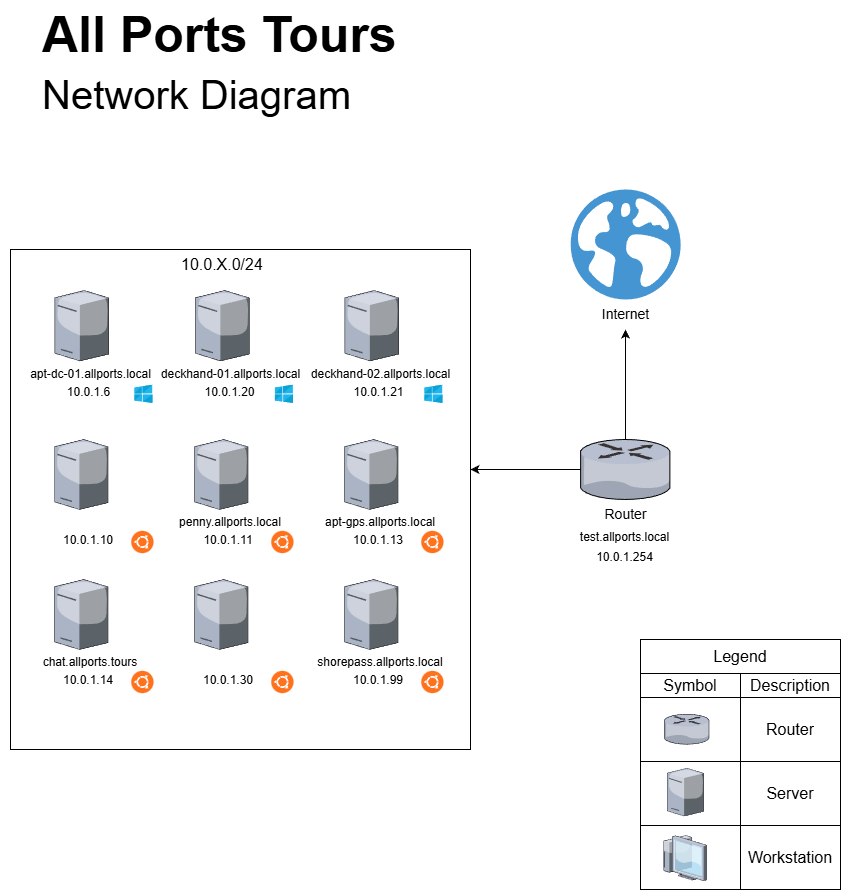
\includegraphics[width=0.95\textwidth]{images/AllPortsToursNetworkDiagram.png}
\end{center}
\renewcommand{\imageBorderWidth}{1pt}